\documentclass[oneside,12pt]{amsart}
%included packages###############################################################
\usepackage{setspace}
\usepackage[english]{babel}
\usepackage{graphicx}
\usepackage{float}
\usepackage{tabularx}
\usepackage{mathtools}
\usepackage{mathrsfs}
\usepackage{amsfonts}
\usepackage{amssymb}
\usepackage{siunitx}
\usepackage{amsthm}
\usepackage{enumitem}
\usepackage{stmaryrd}
\usepackage{multirow}
\usepackage{parskip}
\usepackage{csquotes}
\usepackage{systeme}
\usepackage{caption}
\usepackage{cases}
\usepackage{algorithm}
\usepackage{algpseudocode}
\captionsetup[table]{position=bottom} %UNCOMMENT IF USING CAPTIONS, COMMENTED TO SUPPRESS WARNINGS
\usepackage[backend=biber,style=numeric]{biblatex} %UNCOMMENT IF USING BIBLIOGRAPHY, COMMENTED TO SUPPRESS WARNINGS
\addbibresource{Biblio.bib}
\usepackage[letterpaper, total={6in, 9in}]{geometry}
%Set up graphic path#########
\graphicspath{{./}{}}% You can add the path for the images in the empty brackets 

%Set document dimensions#########################################################
\newdimen\graph
\graph=4.2in
\newdimen\medgraph
\medgraph = 5.3in
\newdimen\smallgraph
\smallgraph = 3in
\newdimen\tinygraph
\tinygraph = 1.5in
\renewcommand{\arraystretch}{1.5}

%Define custom commands here#####################################################
\newcommand{\R}{\mathbb{R}}
\newcommand{\Z}{\mathbb{Z}}
\newcommand{\N}{\mathbb{N}}
\newcommand{\Q}{\mathbb{Q}}
\newcommand{\C}{\mathbb{C}}
\newcommand{\mb}{\mathbf}
\newcommand{\e}[1]{\hat{\mathbf{#1}}}
\newcommand{\esymb}[1]{\hat{\bm{#1}}}
\newcommand{\sub}[1]{_{\text{#1}}}
\newcommand{\lbl}[1]{\stepcounter{equation}\tag{\theequation}\label{#1}}

%Define Custom Operators here ##################################################
\DeclareMathOperator{\arctanh}{arctanh}
\DeclareMathOperator{\const}{const.}

%Define theorems here#################################################################

%Title info#######################################################
\title{A Fine-Grained analysis of XGBoost predicting $T_c$ }
\author{Daniel Briseno}
\date{}
%-Begin Document-%%%%%%%%%%%%%%%%%%%%%%%%%%%%%%%%%%%%%%%%%%%%%%%%%%%%%%%%%%%%%%%%%%%%%%%%%%%%%%%%%%%%%%%%%%
\begin{document}
\maketitle
\section{Introduction}

Superconductors have become increasingly relevant to the development of new technology. Well known applications of superconductors include Magnetic Resonance Imaging (MRI), the Large Hadron Collider at CERN, and proposed superconducing cables which may be able to deliver electricity with no energy loss \cite{hamidieh_data-driven_2018}. 

Another important application of superconductors is the implementation of quantum computers. Quantum computers have recently been shown to posses speed advantages over classical computers, and a scalable implementation of a quantum computer could revolutionize the fields of computer science, computer engineering, and all applications of these disciplines. Among the most promising implementations of quantum computers are those which utilize superconductors to construct their quantum bits (qubits). Notably, the recent demonstration of quantum supremacy by Google used superconducting qubits to achieve their result \cite{supremacy_quantum_2019}. 

Despite the recent demonstration by Google and the best efforts of a large and active research community, a scalable implementation of a quantum computer (and of superconducting technology in general) is restricted by the fact that superconductors have to be cooled to their critical temperature ($T_c$) before they exhibit their superconducting properties. The $T_c$ of a superconductor is often below $77^\circ$K, the boiling temperature of nitrogen\cite{hamidieh_data-driven_2018}. Thus, cooling a system with more than a few hundred cubits is prohibitively expensive. For a sense of scale, Google's celebrated implementation of a quantum computer has 54 qubits, while a typical laptop has an excess of 64 billion bits of RAM.

To this end, the discovery of a superconductor with a high $T_c$ has become an important area of materials science. However finding a physical model of conductivity which can predict the $T_c$ of an arbitrary superconductor remains an unsolved problem, with the most promising approaches relying on heuristics which are often violated in unpredictable ways \cite{hamidieh_data-driven_2018}. Without a theory-based model to predict $T_c$, researchers are turning to Machine Learning algorithms to predict the critical temperature of a material given its atomic properties.

In this report, I will be analyzing the performance of the XGBoost gradient-boosted decision tree algorithm \cite{chen_xgboost_2020} applied to predicting $T_c$ of an arbitrary compound. More specifically, I will be analyzing the performance of XGBoost with hyper-parameters specified by Dr. K. Hamidieh in \cite{hamidieh_data-driven_2018}. 

 Previous attempts at predicting $T_c$ have trained on and predicted $T_c$ for Iron-based, Cuprate, low $T_c$, or $\text{MgB}_2$ based superconductors \cite{owolabi_estimation_2015}\cite{stanev_machine_2018}. Dr. Hamidieh's approach extends $T_c$ prediction to the general class of superconductors (or materials suspected of being superconductors). In his paper, Dr. Hamidieh reports that a properly optimized XGBoost model can predict critical temperature of an arbitrary superconductor with an out-of-sample RMSE of approximately $9.5^\circ$K. 
 
 The data used to train and test this model is the Superconductivity Dataset found in the UCI Machine Learning Repository\cite{noauthor_superconductivity_2018}. It is a collection of 21263 superconductors with 82 features defined for each superconductor. The features of the superconductors are generated from the atomic properties of the elements in the superconductor summarized in Table \ref{tab:elemental_properties} (this table can also be found in \cite{hamidieh_data-driven_2018}).
 
 \begin{table}[h]
     \centering
     \tiny
     \begin{tabularx}{\linewidth}{X X X}
          \hline
          Variable & Units & Description\\
          \hline
        Atomic Mass &Atomic mass units (AMU) &Total proton and neutron rest masses\\
        First Ionization Energy &Kilo-Joules per mole (kJ/mol)&Energy required to remove a valence electron\\
        Atomic Radius & Picometer (pm) &Calculated atomic radius\\
        Density&Kilograms per meters cubed (kg/m3)&Density at standard temperature and pressure\\
        Electron Affinity &Kilo-Joules per mole (kJ/mol) &Energy required to add an electron to a neutral atom\\
        Fusion Heat &Kilo-Joules per mole (kJ/mol) &Energy to change from solid to liquid without temperature change\\
        Thermal Conductivity &Watts per meter-Kelvin (W/(m K)) &Thermal conductivity coefficient $\kappa$\\
        Valence &No units &Typical number of chemical bonds formed by the element\\
        \hline
     \end{tabularx}
     \caption{Elemental properties used to define features used by XGboost to predict $T_c$. }
     \label{tab:elemental_properties}
 \end{table}
 
 For a given superconductor in the data, the atomic properties of the elements which make up that superconductor are combined according to the summary statistics listed below:
 \begin{enumerate}
     \item Mean
     \item Weighted mean
     \item Geometric mean
     \item Weighted geometric mean
     \item Entropy
     \item Weighted entropy
     \item Range
     \item Weighted range
     \item Standard deviation
     \item Weighted standard deviation
 \end{enumerate}
 
 A more in-depth explanation of these summary statistics and their associated formulas can be found in Table 2 of \cite{hamidieh_data-driven_2018}. Apart from these features, the number of elements making up the compound and the $T_c$ of the compound are listed in the data, bringing the total number of features per compound to 82.
 
 While Dr. Hamidieh does specify that XGBoost predicts $T_c$ with an out-of-sample RMSE of $9.5^\circ$K, I will be presenting a finer grained analysis of the performance of XGBoost. More specifically, in the following sections I will attempt to answer:
 
 \begin{enumerate}
     \item How well does XGBoost preform at predicting $T_c$ of Iron, Cuprate, Mercury and $\text{MgB}_2$ based super conductors? Does this performance improve or worsen when trained only on Iron, Cuprate, or $\text{MgB}_2$ based superconductors?
     \item If we divide the testing data by quartiles of $T_c$, how well does XGBoost preform at predicting $T_c$ of compounds in each quartile? Is XGBoost reliable when predicting the $T_c$ of a compound with a high $T_c$?
     \item If we divide the predictions of XGBoost by quartiles of predicted $T_c$, how accurate and precise is XGBoost's prediction when the prediction falls in a given quartile? Is the predicted value of $T_c$ reliable when this predicted value is high?
 \end{enumerate}
 
 The exact metrics used to determine when XGBoost preforms ``well" will be elaborated on in the following section.
 
 \section{Methods}
 
 In this section I will describe the data collection process by first specifying the error statistics collected for predicted $T_c$ values, then describing how these error statistics were collected for any relevant subset of the training and testing data, then finally describing the subsets themselves.
 
 \subsection{Error Statistics}
 
 Let $P$ be the predicted value of $T_c$ and $A$ be the actual value. Then I define the \textbf{raw error} $err$ as $err := P-A$. Note that a negative raw error indicates an under-prediction, and a positive raw error indicates an over-prediction.
 
 This investigation consisted of collecting summary raw error statistics for $T_c$ predictions by XGBoost on relevant subsets of the testing and training data. The error statistics collected are summarized in Table \ref{tab:err_stats}. In the following sections I will call a list of values containing all error statistics in Table \ref{tab:err_stats} an \textbf{error vector}.
 
 \begin{table}[]
     \centering
     \begin{tabularx}{\linewidth}{X X}
     \hline
     Statistic & Description\\
     \hline
       RMSE & The residual mean squared error of predictions \\
        ave\_err  & Raw average of error\\
        std\_err & Standard deviation of raw error values\\
        under\_cnt & Number of under-predictions\\
        over\_cnt & Number of over-predictions\\
        correct\_cnt & Number of exactly correct predictions. Expected to be 0\\
        ave\_under & Average value of under-prediction raw error\\
        ave\_over & Average value of over-prediction raw error\\
        std\_under & Standard deviation of under-prediction raw error\\
        std\_over & Standard deviation of over-prediction raw error\\
        \hline
     \end{tabularx}
     \caption{Summary error statistics collected for predicted $T_c$ values.}
     \label{tab:err_stats}
 \end{table}
 
 \subsection{Data Collection}
 
 There were essentially two types of analysis done which required slightly different approaches to data collection:
 \begin{enumerate}[label=\roman*)]
     \item Collecting error statistics for predicted $T_c$ of compounds with specific actual attributes.
     \item Collecting error statistics for predicted $T_c$ of compounds in different predicted $T_c$ quartiles.
 \end{enumerate}
 It is important to remark on the difference between these two types of analysis. The first focuses analysis on subsets of the training data which are defined by \textit{true} values of the superconductors. For example, one attribute used is whether the compound contains Iron. The second focuses analysis on subsets of the testing data which are defined by the \textit{predicted} value of $T_c$ for a superconductor. 
 
 When doing analysis of type i), collecting a single error vector consisted of:
 \begin{enumerate}
     \item Intersecting the testing and training data with the subset of superconductors under consideration.
     \begin{itemize}
         \item This creates training and testing subsets consisting only of superconductors in the desired subset.
     \end{itemize}
     \item If necessary, retraining the model on the new subsetted training data.
     \begin{itemize}
         \item If no retraining is done, then the default model remains in place. The default model is trained on the whole training data partition before subsetting.
     \end{itemize}
     \item Using the XGBoost model to predict $T_c$ values for superconductors in the subsetted testing data.
     \item Subtracting the actual $T_c$ values from the predicted $T_c$ values to obtain a vector of raw errors
     \item Taking the summary statistics in Table \ref{tab:err_stats} of the raw errors to obtain an error vector.
 \end{enumerate}
 
 This process was carried out 50 times, each time randomly partitioning the superconductor data into 2/3 training data and 1/3 testing data -- and training the XGBoost model on the testing data accordingly. At the end of the 50 trials, this process yielded a matrix of 50 error vectors.
%  \begin{algorithm}[h]
%  \caption{Algorithm to obtain error vector given training data partition, testing data partition, a retraining Boolean flag, and an XGBoost model.}
%  \label{algo:get_err_vect}
%  \begin{algorithmic}
%  \Require{ compute\_statistics := function which given a vector of raw errors, returns an error vector of values defined in Table \ref{tab:err_stats}.}
%   \Function{get\_error\_vector}{ train\_partition: data matrix, test\_partition: data matrix, model: XGBoost model, retrain: Boolean} 
%   \If{retrain}
%     \State Retrain model on train\_partition;
%     \EndIf
%     \State test\_data = test\_partition without column of $T_c$ values;
%     \State actual = select $T_c$ from test\_partition;
%     \State prediction = model.predict(test\_data);
%     \State\Comment{Note that actual and prediction are vectors of $T_c$ values, not single $T_c$ values}
%     \State raw\_err = prediction - actual;
%     \State err\_vector = compute\_statistics(raw\_error);
%     \State \Return err\_vector;
%   \EndFunction
%  \end{algorithmic}
%  \end{algorithm}
 
%  \begin{algorithm}
%  \caption{Algorithm to obtain matrix of transpose error vectors given a subset of superconductors, an empty output matrix, and a retraining flag}
%  \label{algo:get_error_stats_matrix}
%  \begin{algorithmic}
%  \Require{superconductors := data matrix of superconductor data as described in \cite{noauthor_superconductivity_2018}, $\text{partition(data)}$ := function which randomly partitions given data matrix into 2/3 training data and 1/3 testing data -- then returns a tuple of partitions $\langle \text{train,test}\rangle$}.
%  \Function{get\_error\_stats\_matrix}{subset: data matrix, output\_matrix: error vector matrix, retrain: Boolean}
%  \For{i in (1,2,3,...,50)}
%  \State data = partition(superconductors);
%  \State train\_data = data[train];
%  \State model = XGBoost.Train(train\_data);
%  \State train\_partition = train\_data $\cap$ subset;
%  \State test\_partition = data[test] $\cap$ subset;
%  \State err\_vector = get\_error\_vector(train\_partition, test\_partition, model, retrain);
%  \State output\_matrix = output\_matrix.append\_row(err\_vector);
%  \EndFor
%  \State \Return output\_matrix;
%  \EndFunction
%  \end{algorithmic}
%  \end{algorithm}
 
 For analysis of type ii), collecting a single error vector consisted of:
 \begin{enumerate}
     \item Using the XGBoost model to obtain a prediction vector for $T_c$ values of the testing data partition.
     \item Separating prediction vector into predicted $T_c$ quartiles.
     \item For each prediction quartile, subtracting the actual $T_c$ values from the predicted $T_c$ values to obtain a vector of raw errors.
     \item For each vector of raw errors, taking summary statistics in Table \ref{tab:err_stats} to obtain an error vector. 
     \item For each error vector, adding a field to the error vector specifying the prediction quartile for which the summary statistics were taken.
 \end{enumerate}
 This process was carried out 50 times, again, each time randomly partitioning the superconductor data into 2/3 training data and 1/3 testing data, and training the model accordingly. At the end of the 50 trials, this process yielded a matrix of 200 error vectors, 50 vectors per quartile.
 
 \subsection{Subsets Studied}
 Previously, I introduced three questions concerning the performance of XGBoost across three categories: superconductors containing certain elements, superconductors in different true $T_c$ quartiles, and superconductors in different predicted $T_c$ quartiles. 
 
 To this end, there are three classes of subsets under consideration: the element subsets, the true $T_c$ quartiles, and the predicted $T_c$ quartiles.
 
 \subsubsection{The Element Subsets}
 There were four subsets of the data which I call the element subsets. These subsets are: superconductors containing Fe (Iron), containing Cu (Copper), containing $\text{MgB}_2$, and containing Hg (Mercury).
 
 The motivation for the Fe, Cu, and $\text{MgB}_2$ subsets is the body of previous work which applied machine learning to predicting $T_c$ for superconductors containing these compounds. Predicting $T_c$ for superconductors containing these compounds has received priority in the literature due to the practical applications of such superconductors. Thus, it would be useful to characterize how well XGBoost performs on these superconductors.
 
 The motivation for the Hg subset comes from the distribution of $T_c$ values for all superconductors in the dataset, summarized in Figure \ref{fig:Tc_density}. This distribution is extremely skewed towards low values, and is not particularly clustered around a mean. Thus, it seems possible that the model would be biased towards low $T_c$ values. Superconductors containing Hg offer a ``worst case" analysis. Not only do these superconductors have the highest mean $T_c$ of any other elemental class in the dataset, they also have the fourth highest variance \cite{hamidieh_data-driven_2018}. 
 
 \begin{figure}
     \centering
     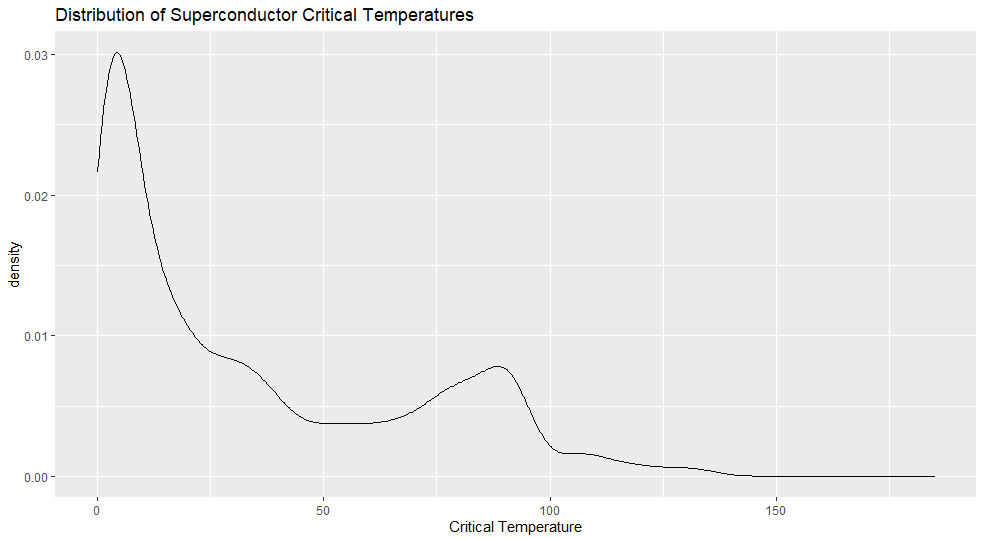
\includegraphics[width=\linewidth]{Tc_dist.png}
     \caption{Density plot of $T_c$ values for all superconductors in dataset.}
     \label{fig:Tc_density}
 \end{figure}
 
 Besides determining the performance of XGBoost on these four subsets, we will analyze any potential benefits of training XGBoost only on compounds of a given element subset when trying to predict $T_c$ values for that subset. The motivation for this is to determine if it would be useful to have separate models for these subsets (as has been done in literature previous to \cite{hamidieh_data-driven_2018}), or if the more generalizable XGBoost model given by Dr. Hamidieh provides sufficient predictive power within these subsets.
 
 Since these subsets are determined by true values of the superconductors, they all use the data collection process i.
 
 \subsubsection{The True $T_c$ Quartiles}
 As one would expect, these subsets simply the superconductor quartiles as defined by the their true $T_c$ values. The motivation for these subsets is again the distribution of $T_c$ values. Since the distribution is skewed towards low values, it is likely that the algorithm under-predicts values in the upper quartiles. 
 
 Identifying this under-prediction (or any other systematic error) may lead to a better optimized algorithm which takes a likely under-prediction of certain superconductors into account.
 
 Since these subsets are determined by the true $T_c$ values of the superconductors, they all use the data collection process i.
 
 \subsubsection{The Predicted $T_c$ Quartiles}
 These subsets are the superconductor quartiles as defined by their \textit{predicted} values of $T_c$. The motivation for this subset is identical to the motivation for the true $T_c$ quartiles, with one distinction. With the predicted $T_c$ quartiles, we will take into account the fact that we do not know the true $T_c$ of an arbitrary conductor. Because of this, implementing a correction term based off of true $T_c$ values would prove difficult, if not impossible.
 
 If a systematic errors can be identified within the predicted $T_c$ quartiles, then implementing a correction term would be easy. We would only need to pick the suitable correction term based off of the observed predicted value of $T_c$.
 
 Since these subsets are determined by the predicted $T_c$ values, they all use the data collection process ii.
 
 \subsubsection{Control Data} In the next section, we will also analyze the performance of XGBoost on a simple 2/3 training and 1/3 testing partition of the superconductor data. The purpose of this analysis is to re-create the results in \cite{hamidieh_data-driven_2018} (specifically the out-of-sample RMSE), and to provide a benchmark for the performance of XGBoost in the other subsets.
 
 The control dataset used data collection process i, with no subsets of the data being taken. Thus, 50 error vectors from 50 random test-train data partitions were collected.
 \section{Results}
 
 In this section, I will present the results of the analysis grouped by the data for which XGBoost predicted $T_c$: the control data, the element subsets, the true $T_c$ quartiles, and the predicted $T_c$ quartiles.
 
 \subsection{Results on the Control Data}
  Figure \ref{fig:control_table} presents average error statistics from the 50 error vectors collected for the control data. Note that the average RMSE is of about $9.5^\circ$ K, thus we can confirm the out-of-sample RMSE presented in \cite{hamidieh_data-driven_2018}.
 
 \begin{figure}[h]
     \centering
     
\includegraphics[width = \linewidth]{control_tbl.png}
     \caption{Average error statistics from the 50 control data error vectors. These error vectors were collected according to data collection process i, with no subsets of the data being taken.}
     \label{fig:control_table}
 \end{figure}

Besides confirming a RMSE of $9.5^\circ$ K, the data in Figure \ref{fig:control_table} also suggests that there was both systemic and random error in the $T_c$ predictions by XGBoost, with XGBoost being biased towards low $T_c$ predictions.

The evidence of systemic error comes from the ave\_err field. If the prediction error was truly random, then errors should be normally distributed (or at least randomly distributed) about a population mean of 0. Thus, we should expect ave\_err to be nearly 0, indicating that XGBoost does not (on average) over nor under predict $T_c$ values. What is observed is that XGBoost, on average, under-predicts $T_c$ by nearly $5^\circ$ K. Moreover, by comparing the number of over-estimates and under-estimates, we can see that XGBoost under-estimates $T_c$ 79.2\% of the time.

Evidence of random error comes from the std\_err field. If the prediction error was only due to bias, we should expect the amount of error in each prediction to be closely clustered and directly proportional to the amount of bias in the model. In practice we can see that the distribution of errors has a standard deviation of about $8^\circ$ K. This suggests that there is some random error present in the model.


 \begin{figure}{}
     \centering
     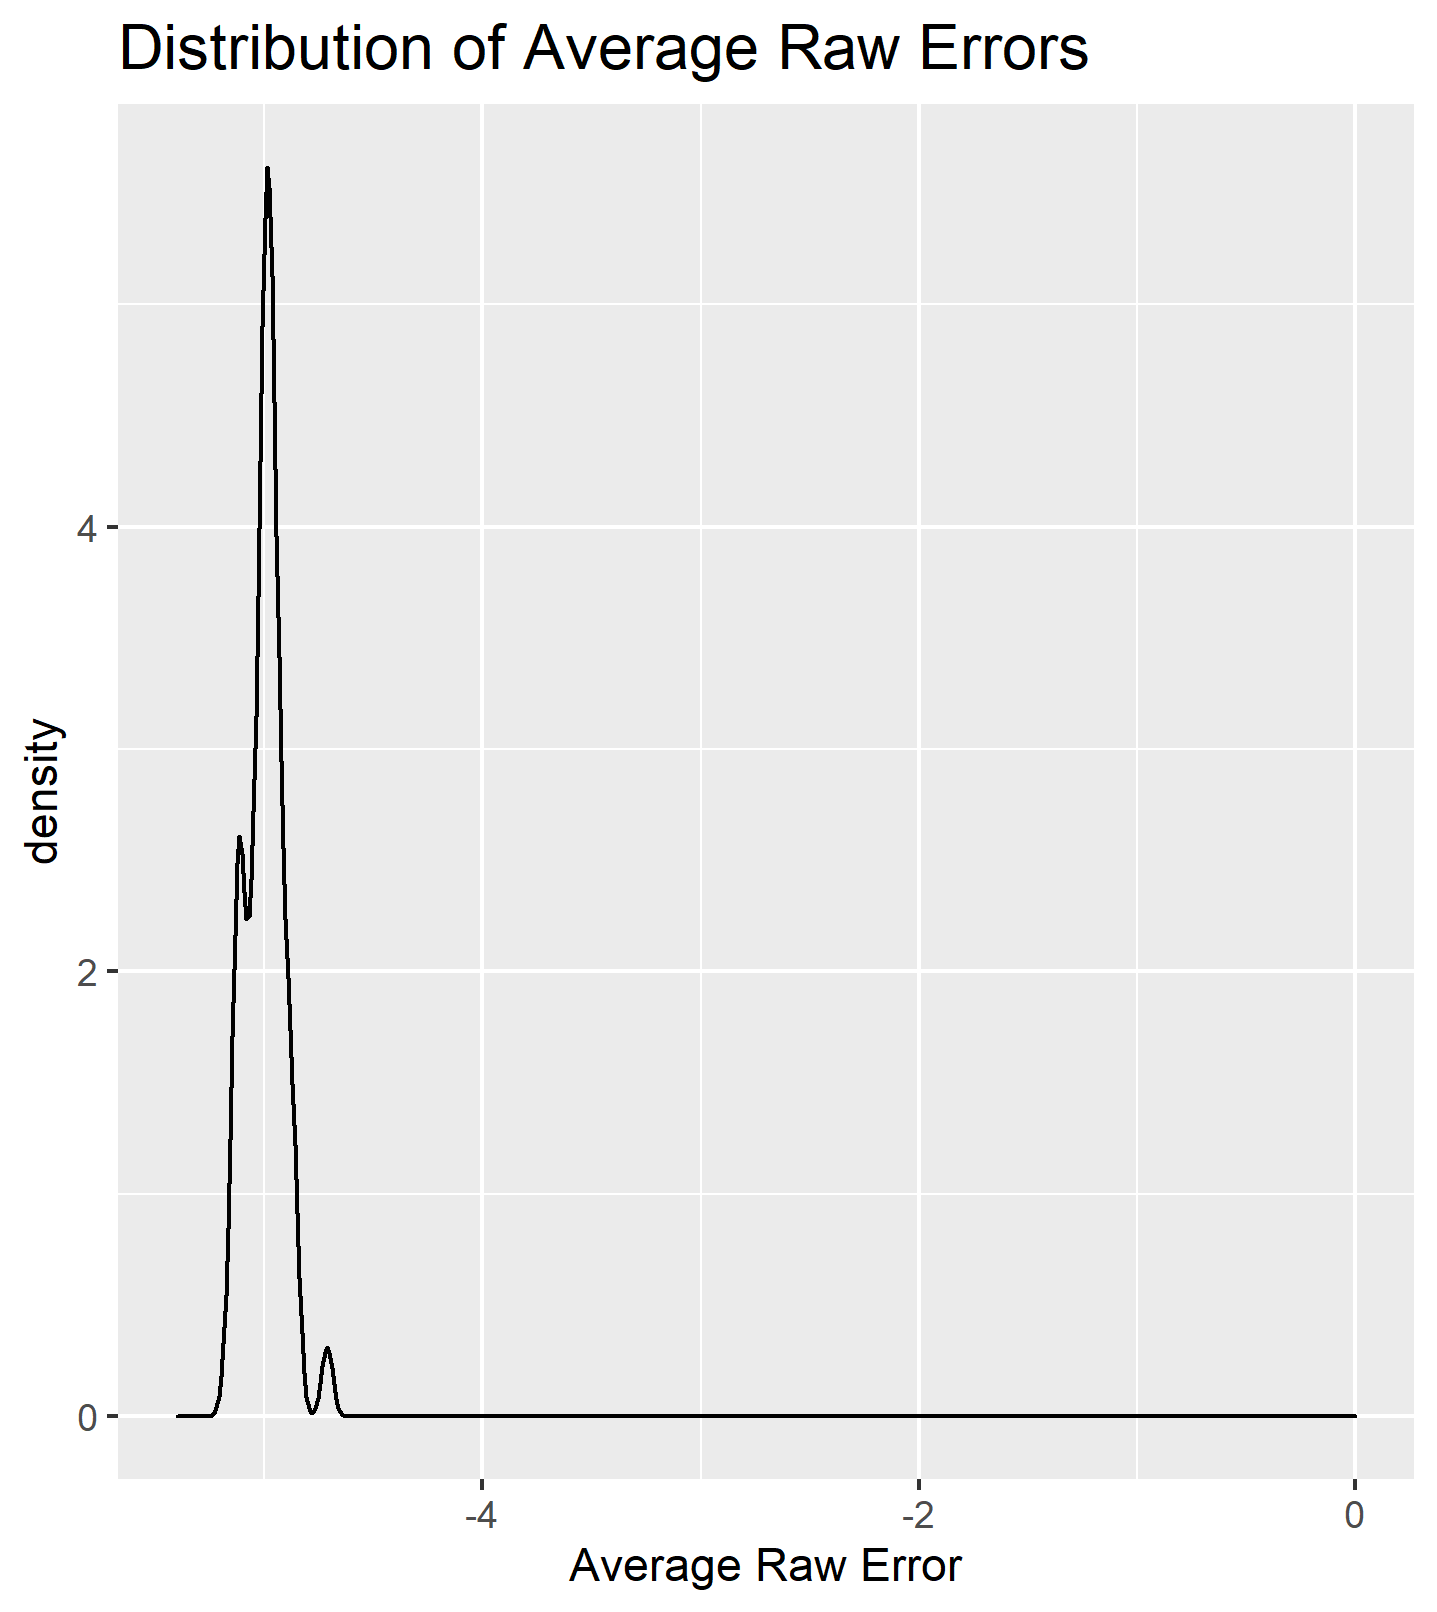
\includegraphics{control_ave_err_density.png}
     \caption{Density plot of average raw errors. Raw error averages were taken from the 50 error vectors collected for the control data.}
     \label{fig:err_denisty}
 \end{figure}

Figure \ref{fig:err_denisty} further supports the hypothesis of an under-prediction bias. Again, if prediction inaccuracies were solely due to random errors, we would expect the average raw errors from each error vector to be normally distributed about 0. What is actually observed is an error distribution closely clustered about $5^\circ$ K, indicating that the errors were not random.

\begin{figure}
    \centering
    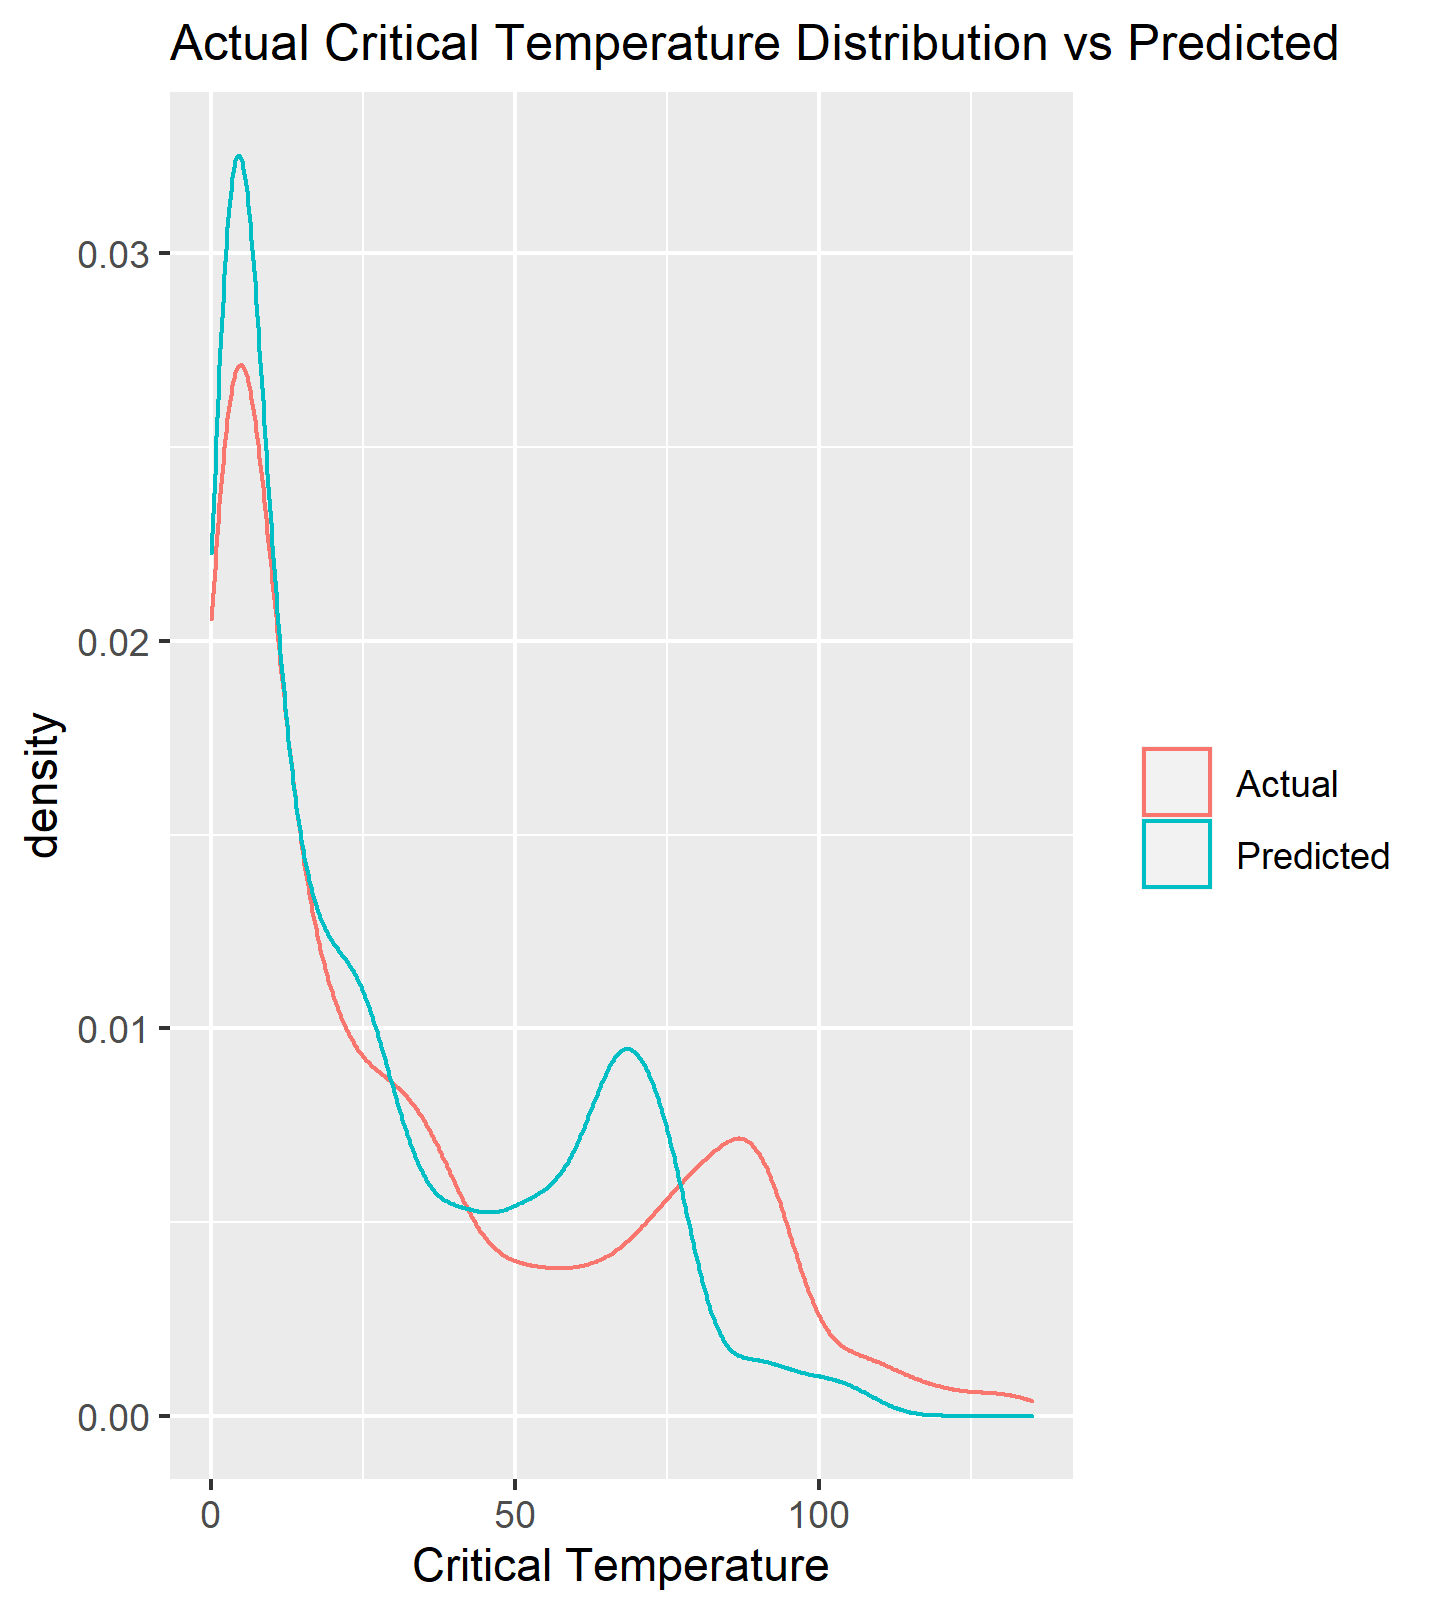
\includegraphics{Actual_vs_Pred_dist.png}
    \caption{Actual test partition $T_c$ distribution plotted alongside the predicted $T_c$ distribution. }
    \label{fig:actual_vs_pred_Tc_dist}
\end{figure}
 
 We can further characterize the nature of the error by comparing the distribution of predicted $T_c$ values to that of the actual $T_c$ values, which is done in Figure \ref{fig:actual_vs_pred_Tc_dist}. We can see two trends:
 \newpage
 \begin{enumerate}
     \item XGBoost correctly finds a sharp peak in the distribution of $T_c$ values near a temperature of $0^\circ$ K. However, XGBoost over-estimates the number of superconductors present in this low $T_c$ cluster.
     \item XGBoost correctly identifies a second small in the distribution with larger $T_c$ values than the low $T_c$ peak. However, XGBoost over-estimates the number of superconductors present in this high $T_c$ cluster, and under-estimates the temperature at which this cluster occurs.
 \end{enumerate}
 
 The bias of the model could, in theory, be corrected by applying a naive correction of $5^\circ$ K to each prediction. However, this may introduce an over-estimation bias in superconductors with low true $T_c$ values. Thus, a finer-grained analysis of the distribution of errors may give a better correction protocol than this naive correction. This is one motivation for the discussion of the $T_c$ quartiles.
 
 \subsection{Results on the Element Subsets} 
 
 Figure \ref{fig:elemental_ntr_tbl} presents average error statistics for the 4 element subsets when XGBoost is trained on a random train partition in the data. Thus, the XGBoost model used to collect these error statistics can be taken to be identical to the model in the control data section.
 
 \begin{figure}
     \centering
     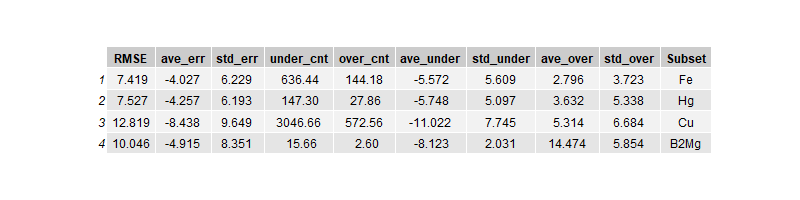
\includegraphics[width = \linewidth]{Elelmental_nrt_ave_tbl.png}
     \caption{Average error statistics from 50 error vectors per element subset. The error vectors were collected according to process i.}
     \label{fig:elemental_ntr_tbl}
 \end{figure}
 
 We can see that XGBoost again has an under-prediction bias across all 4 element subsets, with this bias being most pronounced among the Cu and $\text{MgB}_2$ subsets. 
 
 \begin{figure}[h]
     \centering
     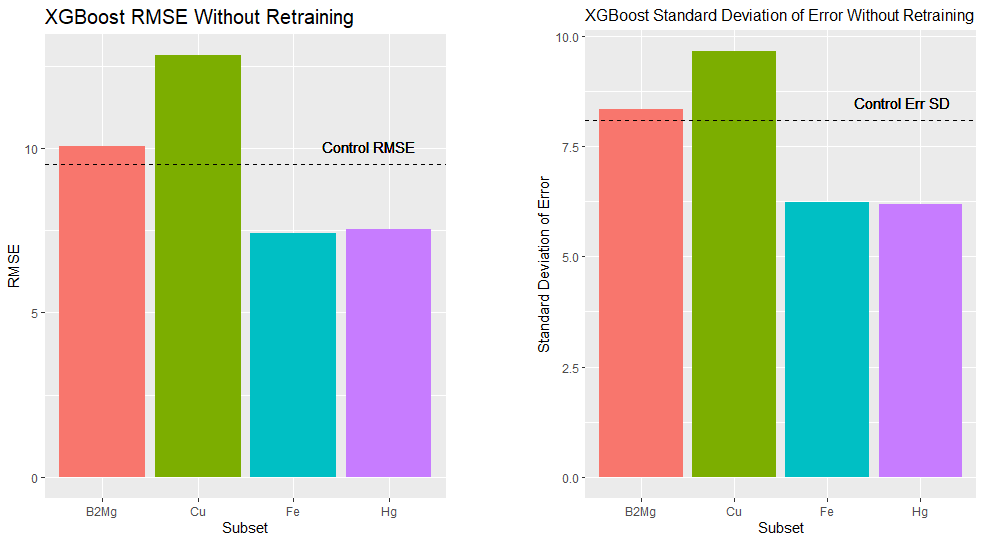
\includegraphics[width=\linewidth]{Elemental_nrt_bxplt.png}
     \caption{RMSE and standard deviation of error on the element subsets without retraining XGBoost on the element subsets. The RMSE and standard deviation of error for the control data are indicated with dashed lines.}
     \label{fig:elemental_nrt_comparsion}
 \end{figure}
 
 Figure \ref{fig:elemental_nrt_comparsion} allows us to compare the performance of XGBoost across the 4 element subsets and against the control data. The RSME and the standard deviation of error are plotted alongside each other, since the RMSE is a measure of the accuracy of the predictions, while the standard deviation gives a sense of the amount of random error present in each set of predictions.
 
 Both plots tell a similar story. XGBoost preformed with greater accuracy and with less random error in the Fe and Hg subsets than in the control data. In contrast, XGBoost had lower accuracy and more random error among the cuprates and the $\text{MgB}_2$ than in the control data. This comes as a mild surprise, since Hg was supposed to serve as a ``worst case" analysis, given the high mean $T_c$ and $T_c$ variance of this subset.
 
 \begin{figure}
     \centering
     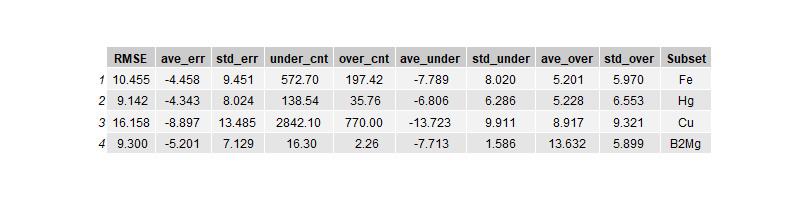
\includegraphics[width = \linewidth]{Elelmental_rt_ave_tbl.png}
     \caption{Average error statistics from 50 error vectors per element subset. The error vectors were collected according to process i. In this case, XGBoost was retrained on the elemental subsets.}
     \label{fig:elemental_rt_tbl}
 \end{figure}
 
 Having established the performance of the control XGBoost model on the element subsets, the element subsets were partitioned into training and testing data, and the XGBoost model was trained and tested accordingly. The results of this process are tabulated in Figure \ref{fig:elemental_rt_tbl} and visualized in Figure \ref{fig:elemental_rt_brplt}.
  \begin{figure}[h]
     \centering
     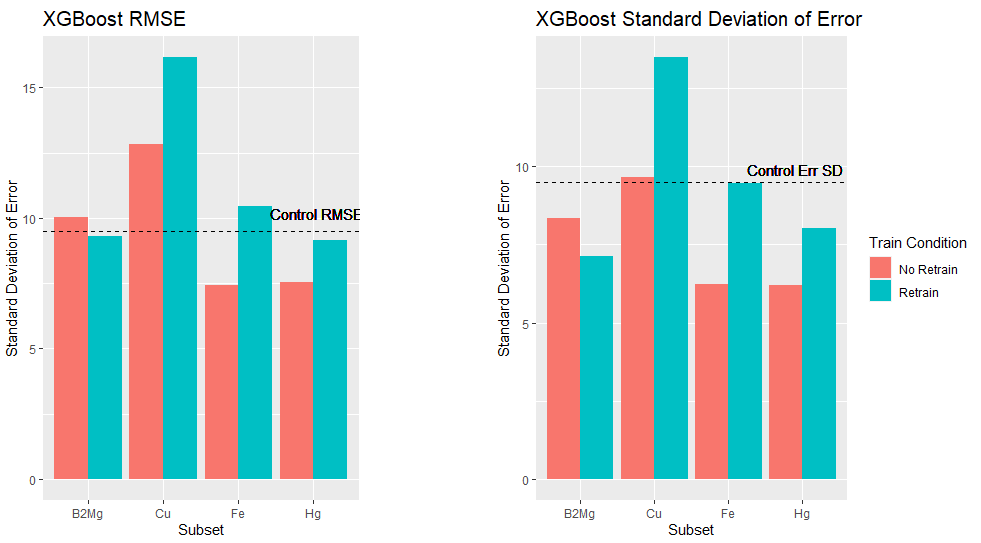
\includegraphics[width=\linewidth]{Elemental_comparison_bxplt.png}
     \caption{Comparison of RMSE and Standard deviation between retraining and no-retraining conditions}
     \label{fig:elemental_rt_brplt}
 \end{figure}
 
 Clearly, both the RMSE and the random error (as quantified by the standard deviation) increased with retraining among all subsets but $\text{MgB}_2$ -- and the improvement in the performance among the $\text{MgB}_2$ superconductors was negligible. Thus, it does not seem to be advantageous to have separate XGBoost models for the different element subsets.
 
 It is interesting to note that the bias quantified by the average random error does not change much between the retraining and non-retraining conditions. The largest difference in the average random error between training conditions was for Cu, with a difference of $0.459^\circ$ K. The fact that the average error in the model changed little despite dramatic changes in the training data indicates that the bias might be a result of the XGBoost model itself rather than the training data. However, more analysis is needed before this claim can be made with high confidence.
 
 I end this section by remarking on the low sample size of the $\text{MgB}_2$ superconductors, with an average testing data partition of 20 superconductors. Thus, any conclusions on the performance of XGBoost on this subset should be taken with reservations.
 
 \subsection{Results on the True $T_c$ Quartiles}
 
 Figure \ref{fig:quart_true_ave_tbl} presents average error statistics for the 4 true $T_c$ quartiles. As expected from the previously observed under-prediction bias, the table shows that XGBoost preforms with increasingly low accuracy and precision for higher $T_c$ quartiles.
 
 \begin{figure}
     \centering
     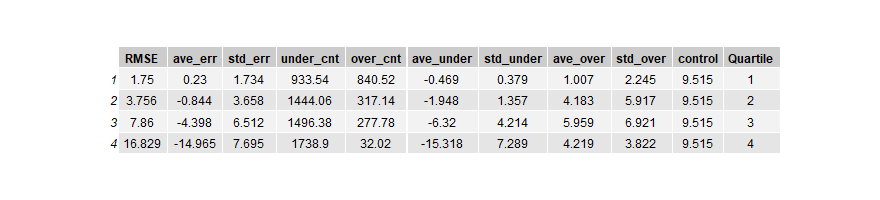
\includegraphics[width = \linewidth]{quart_true_ave_tbl.png}
     \caption{Average error statistics from 50 error vectors collected for each true $T_c$ quartile.}
     \label{fig:quart_true_ave_tbl}
 \end{figure}
 
 \begin{figure}
     \centering
     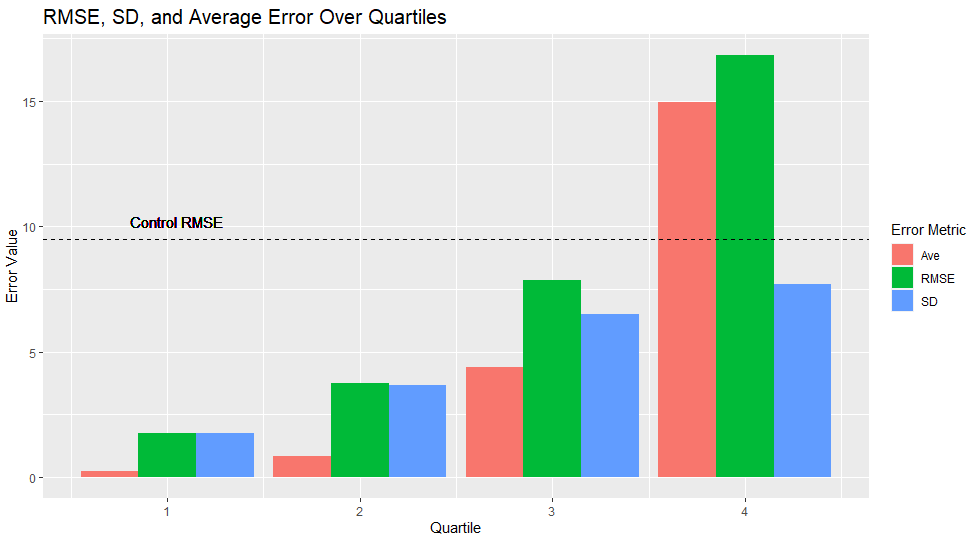
\includegraphics[width=\linewidth]{True_Q_Ave_brplt.png}
     \caption{RSME, standard deviation of error, and the average of raw errors plotted alongside each other for each true $T_c$ quartile.}
     \label{fig:True_Q_Ave_brplt}
 \end{figure}
  
  Figure \ref{fig:True_Q_Ave_brplt} visualizes the bias of the model (as quantified by the average error), the random error (as quantified by the standard deviation of error), and the RMSE of the predicted $T_c$ values among the true $T_c$ quartiles. As expected, the RMSE increases with increasing quartiles. However, we also see that RMSE increases at a rate greater than that of the random error. We also see that the bias increases dramatically with increasing quartiles, indicating that the naive correction term discussed in the control data results is not appropriate.
  
 Figure \ref{fig:True_Q_Ave_brplt} clearly demonstrates the influence of bias and random error in determining the RMSE. In the lowest quartile, we see that average error (and thus -- the bias) is close to zero. Therefore, the errors can be taken to be approximately random and the RMSE is nearly equal to the standard deviation of error, which again quantifies the random error in the predictions. As the average error increases between the quartiles, we see that the RMSE deviates from the standard deviation of error, reflecting an increasing influence of the bias on the RMSE.
  
  This trend culminates in the fourth quartile, where the bias is greater than the random error. Indeed, by looking at the over and under-prediction counts in Figure \ref{fig:quart_true_ave_tbl}, we can see that the model under-predicts $T_c$ for superconductors in the 4th quartile 98\% of the time by an average of $15^\circ$ K.
  
The principle application of this model is to find high $T_c$ superconductors. Therefore, the severe bias in the 4th $T_c$ quartile should be corrected. A possible approach would be adding an average error "penalty" term to the RMSE, and using this combined metric as a target for training XGBoost. At the moment, only RMSE is used as a target.

A second, more easily implemented solution would be to add a correction term to each quartile (with the possible exception of the first) to re-center the error distributions about 0, thus eliminating the bias in each quartile. As discussed before, a problem with this approach is that we do not know the true $T_c$ of a superconductor at the time of prediction. Thus, choosing the appropriate correction term based off of the superconductor's true $T_c$ quartile would be impossible, or at least require a classification model to predict this true quartile in addition to the XGBoost regression model -- a solution which would be computationally expensive.
  
To this end, we turn our attention to the \textit{predicted} $T_c$ quartiles. If the same increase in bias can be observed in the predicted $T_c$ quartiles, then we can choose the appropriate correction term without implementing an additional classification model.

\subsection{Results on the Predicted $T_c$ Quartiles}
Figure \ref{fig:quart_pred_ave_tbl} tabulates the error statistics observed across the predicted $T_c$ quartiles, and these results are visualized in Figure \ref{fig:Pred_Q_Ave_brplt}.
\begin{figure}
    \centering
    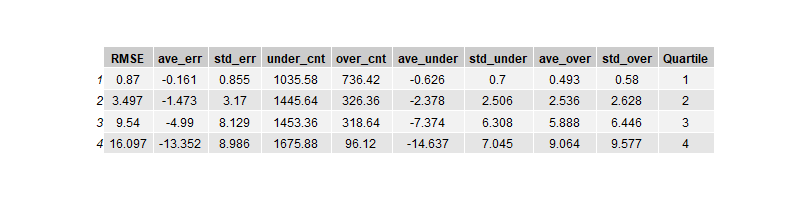
\includegraphics[width=\linewidth]{quart_pred_ave_tbl.png}
    \caption{Average error statistics from 50 error vectors collected for each predicted $T_c$ quartile.}
    \label{fig:quart_pred_ave_tbl}
\end{figure}

\begin{figure}
    \centering
    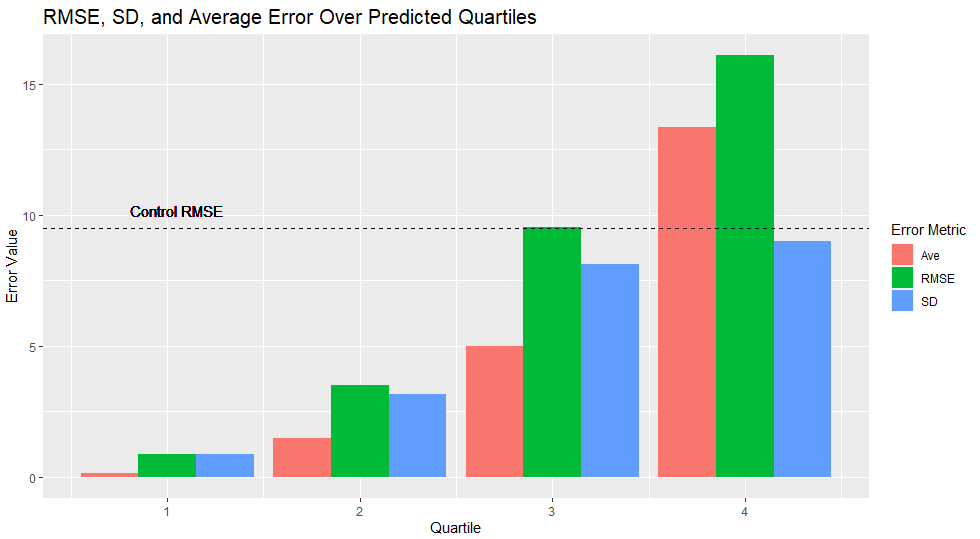
\includegraphics[width = \linewidth]{Pred_Q_Ave_brplt.png}
    \caption{RMSE, standard deviation of error, and the average of raw error plotted alongside each other for each predicted $T_c$ quartile.}
    \label{fig:Pred_Q_Ave_brplt}
\end{figure}

We can confirm that the same trend of increasing bias observed in the true $T_c$ quartiles is present in the predicted $T_c$ quartiles. Therefore, it is possible to add a correction term to the $T_c$ predictions in each quartile based off of the predicted value of $T_c$. Doing so would re-center the error distributions of each quartile at 0, and would make the dominating factor in determining RMSE the random error, which is largely unavoidable and as shown in Figure \ref{fig:Pred_Q_Ave_brplt}, smaller than the bias in the 4th quartile.

\section{Conclusion}
In this report, we analyzed the performance of XGBoost across three categories of superconductors in order to answer the following three questions:

 \begin{enumerate}
     \item How well does XGBoost preform at predicting $T_c$ of Iron, Cuprate, Mercury and $\text{MgB}_2$ based super conductors? Does this performance improve or worsen when trained only on Iron, Cuprate, or $\text{MgB}_2$ based superconductors?
     \item If we divide the testing data by quartiles of $T_c$, how well does XGBoost preform at predicting $T_c$ of compounds in each quartile? Is XGBoost reliable when predicting the $T_c$ of a compound with a high $T_c$?
     \item If we divide the predictions of XGBoost by quartiles of predicted $T_c$, how accurate and precise is XGBoost's prediction when the prediction falls in a given quartile? Is the predicted value of $T_c$ reliable when this predicted value is high?
 \end{enumerate}
 We are now in a position to provide answers to these three questions:
 \begin{enumerate}
     \item XGBoost predicts $T_c$ for Iron, Cuprate, and Mercury based superconductors reasonably well; in each case XGBoost predicts $T_c$ with an RMSE nearly equal to or below the RMSE of $T_c$ predictions for the control data ($9.5^\circ$ K). The performance of XGBoost at predicting $T_c$ for these subsets worsens with retraining on only training data from these three subsets. Thus, it is does not seem advantageous to have separate models for Fe, Cu, and Hg based superconductors
     \begin{itemize}
         \item The opposite effects were shown for $\text{MgB}_2$ based superconductors. XGBoost preformed considerably worse on this subset, and retraining the model improved performance. However, the low sample size of $\text{MgB}_2$ mean that this should be taken with reservations
     \end{itemize}
     \item XGBoost preforms with rapidly decreasing accuracy for increasing $T_c$ quartiles. Thus, the XGBoost model presented in \cite{hamidieh_data-driven_2018} is not reliable for predicting the $T_c$ of a compound with a high true $T_c$ value. However, this decrease in accuracy is primarily driven by an increase in a low-prediction bias in the model. The bias observed in the true $T_c$ quartiles could be corrected by adding an average error penalty term to the training loss function, which at the moment consists of only the RMSE.
     \item As observed in the true $T_c$ quartiles, XGBoost performs with rapidly decreasing accuracy for increasing $T_c$ quartiles. Thus, the $T_c$ value predicted by XGBoost is not reliable when this value is high. Again, this decreasing accuracy is primarily driven by an increasing low-prediction bias among the quartiles. This bias could be corrected by adding a suitable correction to the predicted value of $T_c$, wit this correction depending on the quartile in which the prediction lies.
 \end{enumerate}
 
 By correcting the bias observed in the predicted and observed $T_c$ quartiles could lead to a dramatically better prediction model for superconductors with high $T_c$ values. 
 
 Future work in this direction could include implementing the proposed corrections to XGBoost's predictions, either by adding a average error penalty to the model's loss function, or by adding a correction term to the predicted values of $XGBoost$ which depend on the predicted $T_c$ quartiles.
 
 In addition, the analysis presented in this report relies heavily on summary statistics. The tables presented in the Results section are all averages of 50 or more error vectors. Each error vector is already a set of summary statistics for the raw errors of thousands of predictions. It may be appropriate to directly analyze the distribution of raw errors rather than the distribution of their averages, as was done in this report. Doing so may yield more accurate data about correction terms and the nature of the bias in this model.
 \newpage
\printbibliography
\end{document}
